\section{Cache \weekDoran{3}}
	The cache is completely transparent to the user. It can not explicitly be filled (e.g. using a DMA). The only way to fill the cache is by executing code or data (except for dirty tricks).
	
	The cache is used to store often executed code or data in a closely located storage.
	
	\subsection{Cache Types}
		\begin{longtable}{|>{\bfseries}p{0.3\linewidth}|p{0.65\linewidth}|}
			\hline
			Level 1 Cache
				& Cache that is located closest to the processor. Usually on-chip memory. Also called first level, primary or L1 cache.\\
			\hline
			Level 2 Cache
				& Located downstream of L1 Cache and usually off-chip memory. Also called second level, secondary or L2 cache.\\
			\hline
			Level 3 Cache
				& Located downstream of L2 Cache and usually off-chip memory. Also called third level, tertiary or L3 cache.\\
			\hline	
		\end{longtable}
		%\caption{Cache Types}
		
	\subsection{Cache Behaviour \weekPageDoran{3}{9}}
	
		\begin{table}[H]
			\centering
			\begin{tabular}{|>{\bfseries}p{0.3\linewidth}|p{0.65\linewidth}|}
				\hline
				\multicolumn{2}{|c|}{Controller is looking for a memory item}\\
				\hline
				Cache hit
					& Memory item is found in cache. Controller can be served faster than without cache due to the its proximity to the controller.\\
				\hline
				Cache miss
					& Memory item is not found in cache. Controller is served slower than without Cache due to the checking of the cache before looking in the memory. The \textbf{cache directory} will decide whether a copy of the required datum is in the memory and the \textbf{cache controller} will manage the interaction with system memory, formulated by \textbf{cache policies}. When loading data, it will also be loaded into the cache.\\
				\hline
			\end{tabular}
			%\caption{Cache Behaviour}
		\end{table}
		
	\subsection{Cache Structure \weekPageDoran{3}{9}}
		\subsubsection{Cache Addressing in Direct Mapped Cache}
			\begin{table}[H]
				\centering
				\begin{tabular}{|>{\bfseries}p{0.2\linewidth}|p{0.75\linewidth}|}
					\hline
					Line number
						& Represents the lowest significant bits of the main memory address. It is unique over the whole cache and thus the size depends on the cache. Therefore only one datum of each with the same address in the main memory can be represented in the cache.\\
					\hline
					Address Tag
						& Represents the most significant bits of the main memory address (Complete address without cache line number).\\
					\hline
				\end{tabular}
				%\caption{Cache Addressing in Direct Mapped Cache}
			\end{table} 
			
		\subsubsection {1 Word}
		
			\begin{table}[H]
				\centering
				\begin{tabular}{p{0.15\linewidth}|p{0.06\linewidth}|p{0.06\linewidth}|p{0.06\linewidth}|p{0.2\linewidth}|p{0.2\linewidth}|}
					\cline{2-6}
						\textbf{Line number}
							& \textbf{Valid}
							& \textbf{Dirty}
							& \textbf{Locked}
							& \textbf{Address tag}
							& \textbf{Data}\\
					\cline{2-6}
						0x00
							& 1
							& 1
							& 0
							& Address tag 0
							& Valid data\\
					\cline{2-6}
						0x01
							& 0
							& 1
							& 0
							& N/A
							& Garbage\\
					\cline{2-6}
				\end{tabular}
				%\caption{1 Word cache structure}
			\end{table}	
			
		\subsubsection {2 Word}
		
			\begin{table}[H]
				\centering
				\begin{tabular}{p{0.15\linewidth}|p{0.06\linewidth}|p{0.06\linewidth}|p{0.06\linewidth}|p{0.2\linewidth}|p{0.2\linewidth}|}
					\cline{2-6}
						\textbf{Line number}
							& \textbf{Valid}
							& \textbf{Dirty}
							& \textbf{Locked}
							& \textbf{Address tag}
							& \textbf{Data}\\
					\cline{2-6}
						0x00
							& 1
							& 1
							& 0
							& Address tag 0
							& Valid data\\
					\cline{2-6}
						0x01
							& 
							& 
							& 
							& 
							& Valid data\\
					\cline{2-6}
						0x02
							& 0
							& 1
							& 0
							& N/A
							& Garbage\\
					\cline{2-6}
						0x03
							& 
							& 
							& 
							& 
							& Garbage\\
					\cline{2-6}
				\end{tabular}
				%\caption{2 Word cache structure}
			\end{table}	

	\subsection{Cache Policies}
		\subsubsection{General}
			A \textbf{line fill/update} is when a cache line is updated with a new datum. A \textbf{compulsory line fill/update} is such an update that could not have been avoided using a better cache policy.
			
		\subsubsection{Reading from Cache}
			\begin{table}[H]
				\centering
				\begin{tabular}{|>{\bfseries}p{0.3\linewidth}|p{0.65\linewidth}|}
					\hline
					Look-aside implementation
						& All signals from the CPU are allowed to access main memory, regardless of hit or miss.\\
					\hline
					Look-through / in-line implementation
						& Cache controller decides whether to initiate system memory read/write. Massively reduces CPU-required bandwidth at the cost of \textbf{lookup penalty} (time required to decide that system memory access is required). \\
					\hline
				\end{tabular}
				%\caption{Cache Read Policies}
			\end{table}
			
		\subsubsection{Writing to Cache}
			\begin{table}[H]
				\centering
				\begin{tabular}{|>{\bfseries}p{0.3\linewidth}|p{0.65\linewidth}|}
					\hline
					Write-through policy
						& Both the cache and system memory are updated in order to avoid cache coherence problems.\\
					\hline
					Copy-back policy
						& Only the cache data is updated. This causes cache coherence problems. Simplest method is to set a dirty bit in the cache. When a cache line is replaced the system memory is updated with the new value in the cache (Data is evicted).\\
					\hline
				\end{tabular}
				%\caption{Cache Write Policies}
			\end{table}
			
	\subsection{Cache Locking}
		In some caches, code and data can be locked in the cache. It is different for every cache, in how to achieve this. For the MPC8349e cache looking can be achieved with the following scheme:
		\begin{compactenum}
			\item Invalidate the cache
			\item Load the cache
				\begin{compactitem}
					\item Data
						\begin{compactenum}
							\item Read the data, which shall be locked
						\end{compactenum}
					\item Instructions
						\begin{compactenum}
							\item Load instructions using a speculative fetch
							\item For example a division followed by a branch, which will not be called
							\item The division is used to have enough time to load the speculative fetch
						\end{compactenum}
				\end{compactitem}
		\end{compactenum}
		
	\subsection{Cache Aware Programming}
		\subsubsection{Software Pre-Fetching \weekPageDoran{3}{27}}
			\begin{compactitem}
			  \item Some compilers offer pre-fetching and pre-fetching instruction insertion.
			  \item Manual insertion generally preferred.
			  \item Speed-Up depends largely on algorithm
			\end{compactitem}
			
			\begin{multicols}{2}
				\lstinputlisting[style=CPP]{./src/prefetch.cpp}
			\end{multicols}
		
		\subsubsection{Hardware Pre-Fetching \weekPageDoran{3}{31}}
			A memory access is registered, on the second access the stride (difference between second and first address) is also registered. If the hardware thinks the stride is stable then it starts pre-fetching blocks with this stride.
			
		\subsubsection{Data Access Optimisation \weekPageDoran{3}{34-37}}		
			Cache missed can be minimized with different strategies.			
			\begin{table}[H]
				\centering
				\begin{tabular}{|>{\bfseries}p{0.2\linewidth}|p{0.3\linewidth}|p{0.4\linewidth}|}
					\hline
					Loop Interchange
						& Interchange loop indices. Instead of iterating row-wise iterate column-wise or the other way around.
						& \ \newline 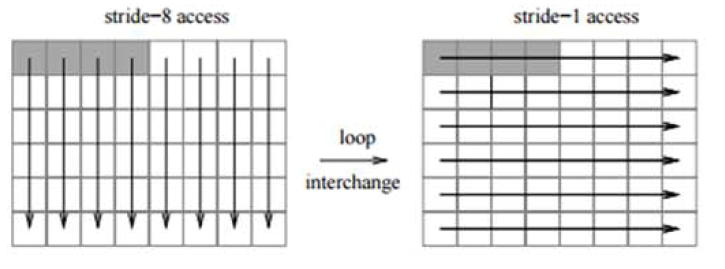
\includegraphics[width=0.4\textwidth]{./pictures/loop_interchange.png}\\
					\hline
					Loop Fusion
						& Combine multiple loops into one. 
						& \\
					\hline
					Loop Blocking/Tiling
						& Instead of iterating column or row wise, iterate in blocks or tiles. (This causes more loops than row or column wise) 
						& \ \newline 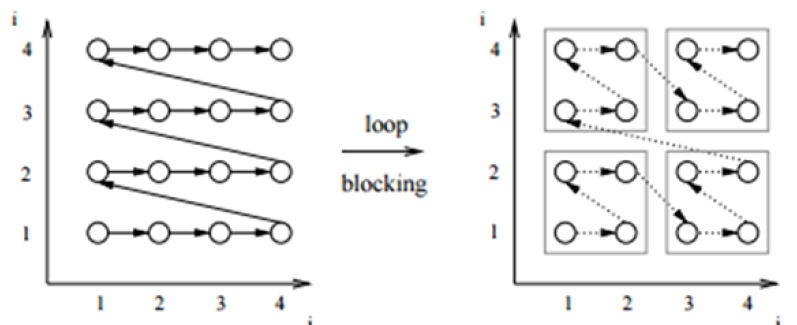
\includegraphics[width=0.4\textwidth]{./pictures/loop_blocking.png}\\
					\hline
				\end{tabular}
				%\caption{Loop Transformations}
			\end{table}
			
	\subsection{Cache Coherence \weekDoran{5}}
		\subsubsection{Cache Snooping Protocol MSI \weekPageDoran{5}{11-14}}
			\begin{tabular}{p{0.475\textwidth}p{0.475\textwidth}}
				\vspace{0pt}
				
				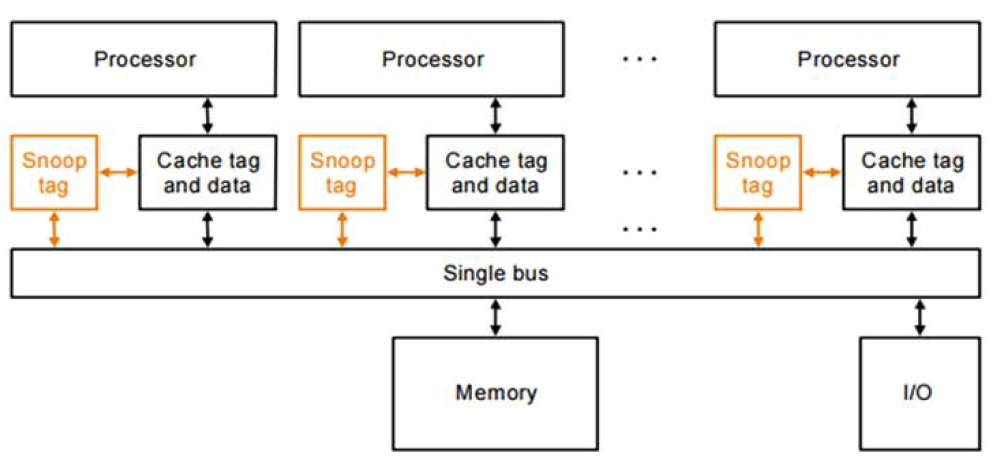
\includegraphics[width=0.5\textwidth]{./pictures/cache_snooping.png}
					& A coherency controller (the snooper) monitors (snoops) the bus transactions and checks if any data modifications are made to data that is present in the snooper's cache. 
					\begin{compactitem}
						\item Cache controller monitors activity on the bus including its own activity
						\item Processor initiates a transaction
						\item If a read transaction on cached line then check for dirty bit and write-back
						\item If a write transaction then invalidate own cache line
					\end{compactitem}\\
			\end{tabular}
			
			\paragraph{General}
			\begin{compactitem}
			  	\item \textbf{Write-invalidate snooping protocol:} When processor writes to shared cache block, the block in all other caches is invalidated through bus snooping. Another possibility is \textbf{Write-update snooping} (uncommon due to high bus traffic). 
			  	\item Single writer, multiple readers
			  	\item Time is divided into epochs
			  	\item In an epoch:
			  		\begin{compactitem}
			  	  		\item Single core may write (rw)
			  	  		\item multiple cores may read (ro)
			  	 	\end{compactitem}
				\item Core reads: send a message to ensure that no other cores are in an rw state
				\item Messages end any rw or ro epoch
				\item When shared data is modified, the changes need to be propagated to all caches which have a copy of the data.
			\end{compactitem}
			
			\paragraph{States}
			\begin{table}[H]\centering
				\begin{tabular}{|>{\bfseries}p{0.1\textwidth}|p{0.36\textwidth}|>{\bfseries}p{0.1\textwidth}|p{0.36\textwidth}|}
					\hline
					\multicolumn{2}{|l|}{\textbf{Memory block states}}
						& \multicolumn{2}{|l|}{\textbf{Cache line states}}\\
					\hline
					Clean
						& In one or more caches and up-to-date in memory.
						& Shared
						& The block is unmodified and exists in read-only state in at least one cache.\\
					\hline
					Dirty
						& In exactly one cache. (updated in cache, not in memory)
						& Invalid
						& The block is either not present in the current cache or has been invalidated. It must be fetched from memory.\\
					\hline
					Uncached
						& In no caches.
						& Modified/\newline\ Exclusive
						& The block has been modified in the cache, and not updated in the memory yet.\\
					\hline
				\end{tabular}
			\end{table}
			
			\begin{figure}[H]\centering
				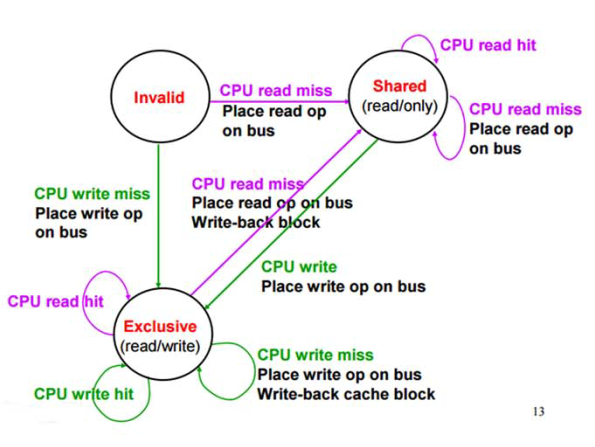
\includegraphics[scale=0.5]{./pictures/MSIProtocol.png}
				%\caption{MSI Protocol cache line states}
			\end{figure}
			
			\paragraph{Transactions}
			
			\begin{tabular}{|>{\bfseries}p{0.15\textwidth}|p{0.8\textwidth}|}
				\hline
				Read miss
					& If another cache contains a dirty value of the datum, it is set to ''valid'' and the copy is sent to the requesting node.\\
					& Values that are initially loaded to cache are set to ''valid''.\\
				\hline
				Write miss
					& If the local cache line is invalid, the CPU experiences a write miss.\\
					& The data is written to the local cache.\\
					& Copies of the datum in other caches are set to ''invalid''.\\ 
				\hline
			\end{tabular}
		
		\subsubsection{Directory based Coherence \weekPageDoran{5}{15-16}}
			\begin{tabular}{p{0.475\textwidth}p{0.475\textwidth}}
				\vspace{0pt}
				
				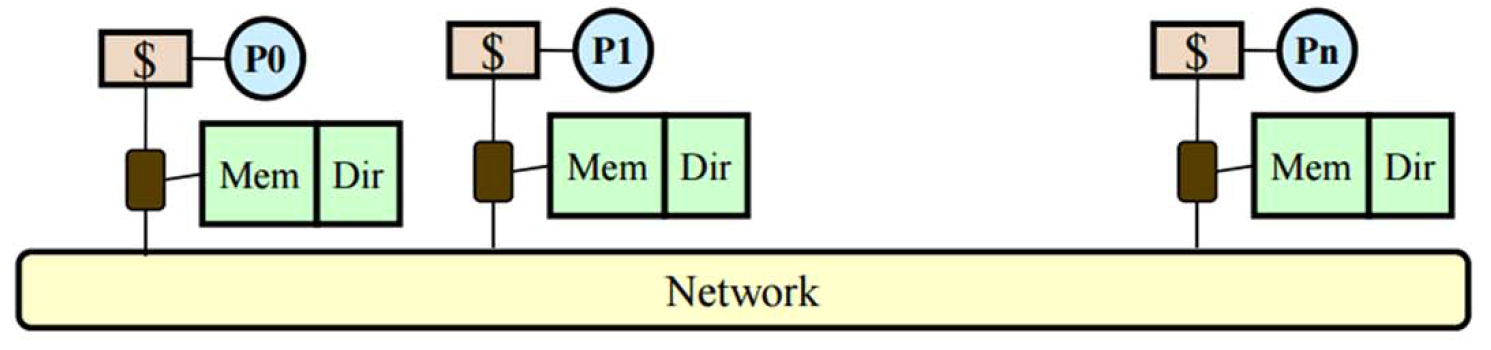
\includegraphics[width=0.5\textwidth]{./pictures/directory.png}
						& A directory keeps track of state an where each copy of a memory block is cached.
					\begin{compactitem}
						\item The directory can be distributed or centralized
						\item The processor consults the directory before loading cache lines
						\item When a line is updated then the directory is consulted to update or invalidate blocks
						\item More scalable than snooping but higher latency
					\end{compactitem}
			\end{tabular}